\documentclass[prl, reprint, twocolumn]{revtex4-1}
\usepackage[utf8]{inputenc}
\usepackage{blindtext}
\usepackage{graphicx}
\usepackage{braket}
\graphicspath{{figures/}}


%\renewcommand{\blindtext}{ }
\begin{document}
	\title{Weakly supervised learning of many-body quantum phases \\ via asymptotic phase classification}
	\date{\today}
	\author{Benjamin Claßen}
	\author{Titus Franz}
	\author{Matthias Weidemüller}
	\affiliation{Physikalisches Institut Heidelberg}
	\begin{abstract}
		
		Main messages:
		\begin{itemize}
			\item Application of the “Confusing Neural Network” method to a Heisenberg model
			\item New method for applying machine learning to a general class of many-body Hamiltonians
			\item Weakly supervised learning of many-body quantum phases via asymptotic phase classification
		\end{itemize}
		
	\end{abstract}
	\maketitle
	
	\section{Introduction}
	\begin{itemize}
		\item Observable based Machine learning for many body systems: Carrasquilla
		\item unsupervised learning of phase diagrams: Nieuwenburg
	\end{itemize}
	\blindtext[2]
	\subsection{The XXZ Heisenberg model}
	\begin{equation}
	H = J\sum_i^L\left(\sigma^x_i\sigma^x_{i+1}+\sigma^y_i\sigma^y_{i+1}+\Delta\sigma^z_i\sigma^z_{i+1}\right) - h_x\sum_i^L\sigma^x_i
	\label{eq:xxz}
	\end{equation}
	\blindtext[2]
	
	\section{The unsupervised confusion scheme}
	Building on the observable-based detection of phase transition as introduced by Carrasquilla et al \cite{Carrasquilla2017}, an unsupervised scheme to scan phase diagrams was introduced by Nieuwenburg et al. \cite{Nieuwenburg2017}.
	While neural networks can natively be used in an unsupervised fashion by using autoencoders for example - these have even been used on many-body problems \cite{Wetzel2017} - the confusion scheme is completely agnostic with regard to the machine learning model used. It is based on the idea that a classifier will perform best if the training data is labeled correctly. By proposing different critical points, labeling the data accordingly and by training a machine learning model on each of these propositions, the classifier is expected to perform best on the proposed critical point closest to the correct critical point.
	
	This approach can be generalized to scan a phase diagram by a sliding window approach\cite{Broecker2017}. Two points $\lambda_1$, $\lambda_2$ within the phase diagram are selected and are proposed to lie within two different phases. A classifier is trained on these two points and the response $p$ when predicting the class of the test data between the 2 training points is recorded. We quantify the probability $P$ that the two points $\lambda_1$ and $\lambda_2$ lie in 2 different phases, i.e. there is a phase transition between the two points as
	
	\begin{equation}
		 P = 2\frac{\int_{\lambda_1}^{\lambda_2} d\lambda |p(\lambda) - 0.5|}{\lambda_2-\lambda_1}
		 \label{eq:P}
	\end{equation}
	
	By scanning the full phase diagram, training a classifier for every point of the discretized space, $P$ displays phase outlines.
	
	There are 2 main parameters to choose for this method: the window width $|\lambda_2-\lambda_1|$ and for phase diagrams of more than one dimension the scan direction has to be considered: If the line segment $\overline{\lambda_1\lambda_2}$ is parallel to a phase boundary, this phase boundary will not be detected.
	Therefore, it was decided to scan once along each axis.
	
	
	
	\subsection{Application of the unsupervised confusion scheme \\ to the XXZ model}
	We simulate the XXZ model's ground state using Matrix Product states\cite{Schollwoeck2011} using the two-site variational ground state search as implemented in the OpenMPS library\cite{Jaschke2018, Wall2012}. The Hamiltonian \ref{eq:xxz} is formulated as Matrix Product Operator for a grid of ($h_x$, $\Delta$) values and the corresponding correlation matrix $\braket{\sigma^i_z\sigma^j_z}$ is recorded.
	
	The machine learning model we use as classifier is a feed-forward, fully connected neural network with just one hidden layer of 100 neurons. Neural networks with more degrees of freedom did not improve the results. The classifier was not trained directly on the simulated correlation matrices, but on the discrete correlation functions $f(r) = \braket{\sigma^i_z\sigma^{i+r}_z}$.
	
	\begin{figure}[h]
		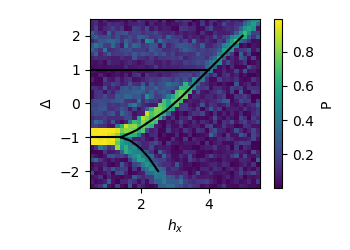
\includegraphics[width=\columnwidth]{3_5_ConfusionPhaseDiagram2D_1_20181214}
		\caption{Application of the confusion scheme to the XXZ model. The scan direction was parallel to the $\Delta$ axis and the window width was set to 0.5. The black line overlay corresponds found using mean field theory\cite{Dmitriev2002}. $P$ corresponds to the probability defined in \ref{eq:P}}
		\label{fig:confusion}
	\end{figure}

	The results of the confusion scheme are presented in \ref{fig:confusion}. We only present the scan parallel to the $\Delta$ axis as the scan parallel to the $h_x$  axis could not reveal any structure parallel to that axis. The two phases for $\Delta = 0$ and high $\Delta$ - values are separated by a crossover. Since the window width is only 0.5, the classifier is not able to reliably discriminate the two phases. But even when increasing the window width to 2, P did not increase at $\Delta=1$.
	
	\section{Weakly supervised learning \\ via asymptotic limits}
	\begin{itemize}
		\item Introduce new approach, which is conceptionally simpler
	\end{itemize}
	\blindtext[2]
	
	
	
	\subsection{Application of the weakly supervised scheme \\ to the XXZ model}
	\begin{itemize}
		\item Plot from thesis: neuron response phase diagram
		\item All phases recognized
	\end{itemize}
	\blindtext[4]
	
	\subsection{Stability of the solution}
	\begin{itemize}
		\item Plot from thesis: Dependence on training data selection
		\item Plot from thesis: Additional or missing phases
	\end{itemize}
	\blindtext[3]
	
	\section{Conclusion}
	\blindtext[3]
	
	
	\bibliography{../mastercode/thesis/library}
	
	
\end{document}